\section[Stückweise Linearisierung]{Stückweise Linearisierung}
\begin{frame}[<+->]
\frametitle{Stückweise Linearisierung}
\begin{itemize}
\item Betrachte nun stückweise lineare Funktionen 
\[
\begin{aligned}
 f&:\R^n \to \R^m, \\
 f&\in \lbrace f_1,\ldots,f_k\rbrace,~f_i(x)=A_ix+b_i~\forall i,~f\text{ global stetig}, \\
 A&\in\R^{m\times n},b\in\R^m
 \end{aligned}
\]
%  \item Betrachte nun $\dot{x} = F(x),~ x_0 = x(0),~F\in C^{0,1}(\R^n)$ (TODO stückweise lineare Funktionen ergänzen)
% \item Es existiert eine Lösung (Filippov)
 \item $f$ ist als \textit{Abs Normal Form} darstellbar $\ldots$
 \end{itemize}
\begin{block}{Abs-Normal Form}
 \begin{equation}
\label{eq:absNormalForm}
  \begin{bmatrix}
   z\\y
  \end{bmatrix}
  =
  \begin{bmatrix}
   c\\b
  \end{bmatrix}
  +
  \begin{bmatrix}
   Z & L\\
   J & Y
  \end{bmatrix}
  \begin{bmatrix}
   x\\|z|
  \end{bmatrix}
 \end{equation}
wobei $c\in \R^s, ~ Z\in \R^{s\times n},~ L\in\R^{s\times s}, ~ b\in\R^m, ~ J\in\R^{m\times n}, ~ Y\in \R^{m\times s}$,\\
$s$ \textit{switching depth}, $z\in \R^s$ \textit{switching Variable} und $L$ strikt untere Dreiecksmatrix
\end{block}
\end{frame}

\begin{frame}[<+->]
\frametitle{Stückweise Linearisierung}
\centering
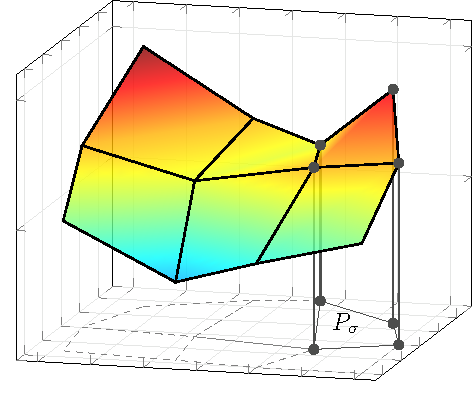
\includegraphics[width=0.65\linewidth]{../dipl_tex/img/tikz/polyhedral_subdevision.pdf}
\end{frame}

\begin{frame}[<+->]
\frametitle{Stückweise Linearisierung}
\begin{itemize}
 \item $\ldots$ und kann benutzt werden, um verkettet stückweise glatte Funktionen 
 \[
 \begin{aligned}
   f&:\R^n \to \R^m, \\
 f&\in \lbrace f_1,\ldots,f_k\rbrace,~f_i(x) \in C^1(\R^n)~\forall i,~f \text{ global stetig}\\
 &\text{verknüpft durch }\varphi_i \in \lbrace +,*,sin,exp,abs ,\ldots\rbrace                                                                
 \end{aligned}
 \]
an einer Entwicklungsstelle $\xo$ zu approximieren
%  \item Verkettet stückweise glatte Funktionen: stückweise definierte, stetige Funktionen, dessen Auswahlfunktionen stetig differenzierbar sind
% \item Diese Approximation heißt \textit{stückweise Lineariserung} an der Stelle $\xo$ und hat die Form 
% \[
%  F(\xo) + \Delta F(\xo; x-\xo)
% \]
% welche auch als \textit{tangent mode} bezeichnet wird.
\end{itemize}
% \begin{block}{Eigenschaften der Stückweisen Linearisierung}
%  \begin{itemize}
%   \item Blub
%   \item blob
%   \item Blubber
%  \end{itemize}
% \end{block}
\end{frame}

\begin{frame}[<+->]
\frametitle{Stückweise Linearisierung}
\begin{figure}
\centering
% \resizebox{.9\linewidth}{!}{ \documentclass{standalone}
\IfStandalone{
	\usepackage{pgfplots,pgfplotstable}
	\usetikzlibrary{external}
	\newcommand{\fromRoot}[1]{../#1}
	\newcommand{\D}{\Delta}
	\pgfplotsset{compat=1.9}
}{%
}

\begin{document}
\tikzsetnextfilename{piecewise_linearization}
\begin{tikzpicture}
\def\xo{-1};
\pgfmathdeclarefunction{f1}{1}{%
	\pgfmathparse{-(6/10)*(#1+2)^2}%
}
\pgfmathdeclarefunction{f2}{1}{%
	\pgfmathparse{3*( #1+sin((11/10)*deg(#1)) )}%
}
\pgfmathdeclarefunction{tf1}{1}{%
	\pgfmathparse{-1.2*(#1+1)-0.6}%
}
\pgfmathdeclarefunction{tf2}{1}{%
	\pgfmathparse{4.49687*(#1+1)-5.67362}%
}
\begin{axis}[
	height=0.45\textheight,
	axis y line = none,
	axis x line = bottom,
	xmin=-4,xmax=4,
	xtick = \empty,
	ytick = \empty,
	extra x ticks = {\xo},
	extra x tick labels={\(\mathring x\)},
	extra x tick style = {grid=major},
	domain=-4:4,
	samples=500,
]
\addplot[red!60!white] {f1(x)} 
	[yshift=2pt] 
	node[anchor=south,pos=0.8] {$F_1$};
\addplot[blue!60!white] {f2(x)} 
	node[anchor=south,pos=0.1] {$F_2$};
\addplot[black,yshift=1pt] {max(f1(x),f2(x)} 
	node[anchor=south,pos=0.2] {$F = \max(F_1,F_2)$};

\addplot[red!60!white,very thin] {tf1(x)} 
	node[anchor=south,pos=0.75,sloped] {$\mathring F_1 + F_1'(\mathring x)\D x$};
\addplot[blue!60!white,very thin] {tf2(x)} 
	node[anchor=north,pos=0.15,sloped] {$\mathring F_2 + F_2'(\mathring x)\D x$};
\addplot[black,very thin,yshift=1pt] {max(tf1(x),tf2(x)} 
	node[anchor=south,pos=0.75,sloped] {$\mathring F + \D F(\mathring x;\D x)$};
%\addplot [color=black,only marks,mark=*] coordinates { (-1,-0.6) };
%\addplot [color=black,only marks,mark=*] coordinates { (-1,-5.67362) };
\end{axis}
\end{tikzpicture}

 
\end{document}
 }
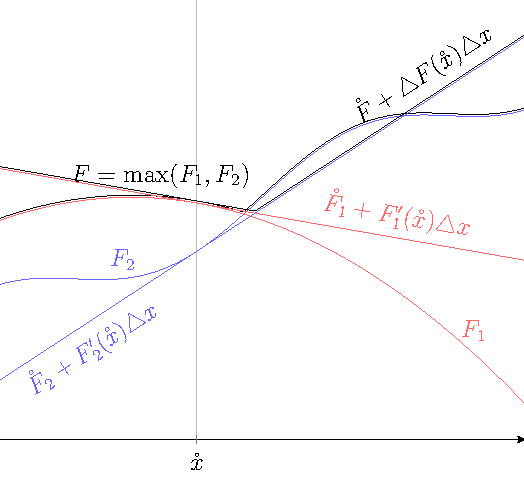
\includegraphics[width=0.65\linewidth]{../dipl_tex/img/tikz/piecewise_linearization.pdf}
\end{figure}
\end{frame}

\begin{frame}[<+->]
\frametitle{Stückweise Linearisierung}
\begin{block}{Eigenschaften}
 \begin{itemize}
  \item Approximation 2. Ordnung: \[\|F(x) - F(\xo)- \Delta F(\xo;x-\xo)\| \leq \gamma \|x-\xo\|^2\]
  \item Inkrementfunktion 
    \[\Delta F(\xo;\Delta x) = F'(\xo;\Delta x)~ \text{für } \Delta x \leq \rho(\xo)\]
  
 \end{itemize}
\end{block}
\begin{block}{AD}
 Automatische Berechnung der Stückweisen Linearisierung in Abs Normal Form mittels zusätzlicher AD Regel:
 \[
%   \Delta v_i = (v_j \neq 0)?sign(v_j )\Delta v_j : abs(\Delta v_j) \text{ für } v_i = abs(v_j), j\prec i
    \Delta v_i =\abs(v_j + \Delta v_j) - v_i \text{ für } v_i = abs(v_j), j\prec i
 \]
\end{block}

\end{frame}
